\chapter{Households}
\index{Households%
@\emph{Households}}%

  \section{Demographics}
    A measure $\omega_{1,t}$ of individuals with heterogeneous working ability $e \in\mathcal{E}\subset\mathbb{R}_{++}$ is born in each period $t$ and live for $E+S$ periods, with $S\geq 4$.\footnote{Theoretically, the model exposition of the model works without loss of generality for $S\geq 3$. However, because we are calibrating the ages outside of the economy to be one-fourth of $S$ (e.g., ages 21 to 100 in the economy, and ages 1 to 20 outside of the economy), we need $S$ to be at least 4.} The population of age-$s$ individuals in any period $t$ is $\omega_{s,t}$. Households are termed ``youth'', and do not participate in market activity, during ages $1\leq s\leq E$. The households enter the workforce and economy in period $E+1$ and remain in the workforce until they unexpectedly die or live until age $s=E+S$.\footnote{We model the population with households age $s\leq E$ outside of the workforce and economy in order most closely match the empirical population dynamics.} The population of agents of each age in each period, $\omega_{s,t}$, evolves according to the following function,
    \begin{equation}\label{EqPopLawofmotion}
      \begin{split}
        \omega_{1,t+1} &= \sum_{s=1}^{E+S} f_s\omega_{s,t}\quad\forall t \\
        \omega_{s+1,t+1} &= (1 + i_s - \rho_s)\omega_{s,t}\quad\forall t\quad\text{and}\quad 1\leq s \leq E+S-1
      \end{split}
    \end{equation}
    where $f_s\geq 0$ is an age-specific fertility rate, $i_s$ is an age-specific immigration rate, $\rho_s$ is an age specific mortality hazard rate,\footnote{The parameter $\rho_s$ is the probability that a household of age $s$ dies before age $s+1$.} and $1+i_s-\rho_s$ is constrained to be nonnegative. The total population in the economy $N_t$ at any period is simply the sum of individuals in the economy, the population growth rate in any period $t$ from the previous period $t-1$ is $g_{n,t}$, $\tilde{N}_t$ is the working age population, and $\tilde{g}_{n,t}$ is the working age population growth rate in any period $t$ from the previous period $t-1$.
    \begin{equation}\label{EqPopDef}
      N_t\equiv\sum_{s=1}^{E+S} \omega_{s,t} \quad\forall t
    \end{equation}
    \begin{equation}\label{EqPopGrowth}
      g_{n,t+1} \equiv \frac{N_{t+1}}{N_t} - 1 \quad\forall t
    \end{equation}
    \begin{equation}\label{EqPopWkDef}
      \tilde{N}_t\equiv\sum_{s=E+1}^{E+S} \omega_{s,t} \quad\forall t
    \end{equation}
    \begin{equation}\label{EqPopWkGrowth}
      \tilde{g}_{n,t+1} \equiv \frac{\tilde{N}_{t+1}}{\tilde{N}_t} - 1 \quad\forall t
    \end{equation}


  \section{Households}
  Consumer's are forward-looking, intertemporal optimizers.  Their objective is the maximize the expected, discounted value of lifetime utility.  Expectations are taken over mortality risk, the only source of uncertainty in the model.  Individuals are heterogenous with repeat to age and lifetime income group.  We define the expected, discounted lifetime utility at time $t$ for an individual in lifetime income group $j$ and age $s$ to be $U_{j,s,t}$.  We assume that utility is additively separable across periods and thus write expected, discounted lifetime utility as:
    \begin{equation}\label{EqUtilMax}
      \begin{split}
        &U_{j,s,t} = \sum_{u=0}^{E+S-s}\beta^u\left[\prod_{v=s-1}^{s+u-1}(1-\rho_v)\right] u\left(c_{j,s+u,t+u},n_{j,s+u,t+u},b_{j,s+u+1,t+u+1}\right) \\
        &\text{where}\quad \rho_{s-1}=0 \\
        &\text{and} \quad u\left(c_{j,s,t},n_{j,s,t},b_{j,s+1,t+1}\right) = \frac{\left(c_{j,s,t}\right)^{1-\sigma} - 1}{1-\sigma} ... \\
        &\qquad\qquad + e^{g_y t(1-\sigma)}\chi^n_s\left(b\left[1 - \left(\frac{n_{j,s,t}}{\tilde{l}}\right)^\upsilon\right]^\frac{1}{\upsilon} + k\right) + \rho_s\chi^b\frac{\left(b_{j,s+1,t+1}\right)^{1-\sigma} - 1}{1-\sigma} \\
        &\quad\quad\quad\quad\quad\quad\quad\quad\quad\quad\quad\quad\quad\quad\quad\quad\quad\quad\quad\forall j,t\quad\text{and}\:E+1\leq s\leq E+S
      \end{split}
    \end{equation}

\noindent\noindent The parameter $\beta\in(0,1)$ represents the individual's rate of time preference.  The quantities $c_{j,s,t}$, $n_{j,s,t},$ and $b_{j,s,t}$ are total consumption of a composite consumption good, labor supply, and asset holdings, respectively.  The parameter $\sigma \geq 1$ is the coefficient of relative risk aversion, $\upsilon$ is a measure of the elasticity of labor supply, and $\tilde{l}$ is the total time endowment of the individual.  The utility weight for the disutility of labor is given by the age-dependent parameters $\chi^{n}_{s}$.  The parameter $g_y$ is a constant growth rate of labor augmenting technological progress, which we explain in more detail in the firm's problem .\footnote{The term with the growth rate $e^{g_y t(1-\sigma)}$ must be included in the period utility function because consumption and bequests will be growing at rate $g_y$ and this term stationarizes the individual Euler equation by making the marginal disutility of labor grow at the same rate as the marginal benefits of consumption and bequests.  This is the same balanced growth technique as that used in \citet{MertensRavn:2011}.}  The disutility of labor term in the utility function looks nonstandard, but is simply the upper quadrant of an ellipse that closely approximates the standard constant relative risk aversion utility of leisure functional form.\footnote{Appendix \ref{AppEllipseUtil} describes how the elliptical function closely matches the more standard utility of leisure of the form $\frac{(\tilde{l}-n_{j,s,t})^{1-\eta} - 1}{1-\eta}$. The parameters $b$ and $k$ are the scale and shift parameters of describing the elliptical form.  This elliptical utility function forces an interior solution that automatically respects both the upper and lower bound of labor supply, which greatly simplifies the computation of equilibrium.  For a more in-depth discussion see \citet{EvanPhillips:2015}} The utility weight on bequests (both intentional and accidental) is given by $\chi^{b}$.

 \begin{figure}[htb]\centering \captionsetup{width=4.0in}
\caption{\label{fig:hh_tree}\textbf{Summary of the Individual Problem}}
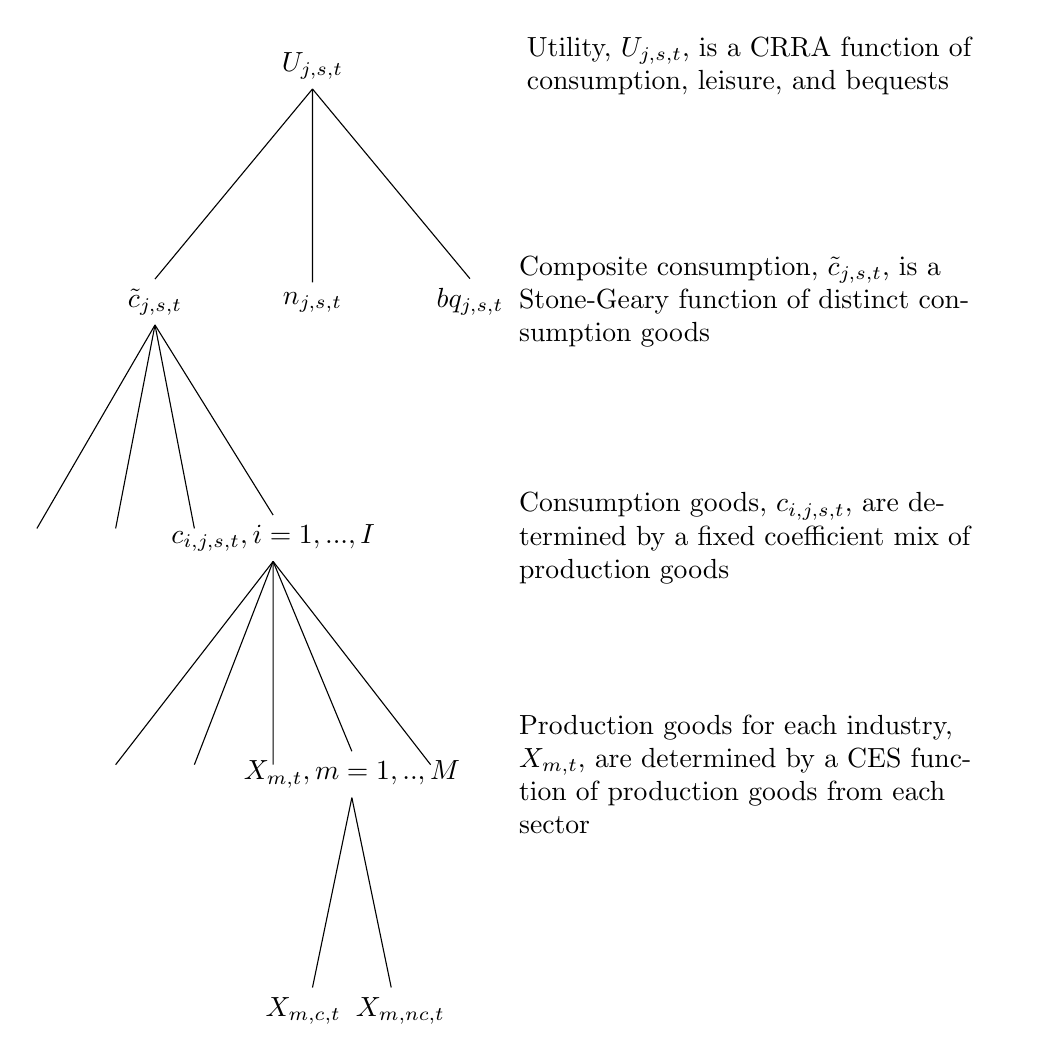
\begin{tikzpicture}
\tikzstyle{every node}=[auto,every node/.style={rectangle,draw, text centered, text width=1.3cm,minimum height=0.8cm },node distance=3cm]
\tikzset{%
level 1/.style={sibling distance = 2cm, level distance=3cm,edge from parent path={(\tikzparentnode.south) -- (\tikzchildnode.north)}},
level 2/.style={sibling distance = 1cm,level distance=3cm}
%level 4/.style={sibling distance = 1.1cm,level distance=3cm}
}
  \node (0){$U_{j,s,t}$}
    child {node (1) {$\tilde{c}_{j,s,t}$}
    child {node {}}
    child {node {}}
    child {node {}}
    child {node (2){$c_{i,j,s,t}, i=1,...,I$}   
child {node (3) {}}
            child {node {}}
            child {node {}}
            child {node {$X_{m,t}, m=1,..,M$}       
             child {node {$X_{m,c,t} \ \ $}}
             child {node {$\ \ X_{m,nc,t}$}}}
             child {node {}}
                        }
                  }
child {node {$n_{j,s,t}$}}
child {node {$bq_{j,s,t}$}} ;

\node at (0) [xshift=+2.6cm,right,draw=none, text width=6cm]{Utility, $U_{j,s,t}$, is a CRRA function of consumption, leisure, and bequests};
\node at (1) [xshift=+4.5cm, right,draw=none, text width=6cm]{Composite consumption, $\tilde{c}_{j,s,t}$, is a Stone-Geary function of distinct consumption goods};
\node at (2) [xshift=+3.0cm, right,draw=none, text width=6cm]{Consumption goods, $c_{i,j,s,t}$, are determined by a fixed coefficient mix of production goods };
\node at (3) [xshift=+5.0cm, right,draw=none, text width=6cm]{Production goods for each industry, $X_{m,t}$, are determined by a CES function of production goods from each sector};
\end{tikzpicture}
\end{figure}


    Households choose consumption of a composite consumption good, $c_{j,s+u,t+u}$, labor supply, $n_{j,s+u,t+u},$ and asset holdings, $b_{j,s+u+1,t+u+1}$, to maximize the expected, discounted, lifetime utility subject to their per-period budget constraint.  Total consumption of the composite good is made up of discretionary consumption, $\tilde{c}_{j,s,t}$, and minimum required purchases of each consumption good, $\bar{c}_{i,s}$.  Thus the consumer's choice is over $\tilde{c}_{j,s,t}$, which together with the minimum required purchases equal determine total composite consumption: $c_{j,s,t}=\tilde{c}_{j,s,t}+\sum_{i=1}^{I}c_{i,s}$.  It is therefore the case that there minimum required purchases affect the household's ability to smooth consumption over time.  We discuss the composite consumption good in more detail in Section \ref{sec:subutil}.  This composite good is age dependent, thus the price of the composite consumption good varies with age $s$.  We denote the gross-of-tax price of the composite consumption good for households of age $s$ in period $t$ as $\tilde{p}_{s,t}$ and the gross-of-tax price for good $i$ at time $t$ as $p_{i,t}$. The households' per period budget constraint is:
    
    \begin{equation}\label{EqBC}
      \begin{split}
        \sum_{i=1}^{I} p_{i,t}\bar{c}_{i,s} + \tilde{p}_{s,t}\tilde{c}_{s,t} + b_{j,s+1,t+1} \leq \left(1 + r_t\right) b_{j,s,t} + w_t e_{j,s}&n_{j,s,t} + \frac{BQ_{j,t}}{\lambda_j\tilde{N}_t} - T_{j,s,t} \\
        \quad\text{where}\quad b_{j,s,1} = 0 \\
        &\text{for} \quad E+1\leq s \leq E+S \quad \forall j,t
      \end{split}
    \end{equation}

\noindent\noindent Here, $r_{t}$ and $w_{t}$ are the real interest rate and the wages rate on a unit of effective labor.  The variable $e_{j,s}$ denotes the effective labor units of an individual from lifetime income group $s$ and age $j$.  An individual's labor income is thus determined by her choice of $n_{j,s,t}$ units of labor times her measure of effective labor units, $e_{j,s}$, times the wage per unit of effect labor.  An individuals effective labor units vary over the life-cycle, as the age subscript implies.  $BQ_{j,t}$ denote aggregate bequests left from those in lifetime income group {j} at time {t}.  We divide this number by the number of individuals in lifetime income group $j$ at time $t$, given by $\lambda_{j}\tilde{N}_{t}$, to determine the amount of bequests received by each household in lifetime income group $j$.\footnote{This distribution of bequests is just place holder. The goal is to find suitable data to calibrate the process describing the transmission of bequests between individuals of different ages and lifetime income groups.}  The last term in the budget constraint, $T_{j,s,t}$ are total taxes paid by the individual.  These include all non-consumption taxes and are based on tax functions for separate tax sources that we estimate based on a microsimulation model.  We discuss the parameterization and calibration of these functions below. 

    The Lagrangian for the individual's problem can be written as:
     \begin{equation}\label{eqn:hh_prob_lagrangian}
      \begin{split}
     \mathcal{L} =  \max_{\left\{ \substack{\tilde{c}_{j,s+u,t+u},\\\ {n}_{j,s+u,t+u},\\\ {b}_{j,s+u,t+u}}\right\}_{u=0}^{E+S-s}}  &  \sum_{u=0}^{E+S-s}\beta^u\left[\prod_{v=s-1}^{s+u-1}(1-\rho_v)\right]  \frac{\left(c_{j,s+u,t+u}\right)^{1-\sigma} - 1}{1-\sigma} + ...\\
  &   e^{g_y t(1-\sigma)}\chi^n_s+u\left(b\left[1 - \left(\frac{n_{j,s+u,t+u}}{\tilde{l}}\right)^\upsilon\right]^\frac{1}{\upsilon} + k\right) + \rho_s\chi^b\frac{\left(b_{j,s+u+1,t+u+1}\right)^{1-\sigma} - 1}{1-\sigma}  +... \\
       & \lambda_{j,s+u,t+u}\left\{ (1+r_{t+u})b_{j,s+u,t+u} + w_{t+u}e_{j,s+u}n_{j,s+u,t+u}+\frac{BQ_{j,t+u}}{\lambda_{j}\tilde{N}_{t+u}}-T_{j,s+u,t+u} -.... \right.\\
       & \left. \sum_{i=1}^{I}p_{i,t+u}\bar{c}_{i,s+u}-\tilde{p}_{s+u,t+u}\tilde{c}_{j,s+u,t+u} -b_{j,s+u+1,t+u+1} \right\}
        \end{split}
    \end{equation}
    
    
    
\noindent\noindent taking derivatives with respect to $\{\tilde{c}_{j,s,t},n_{j,s,t+u},b_{j,s,t+1}\}$ gives us the necessary conditions for each $j,s$ and $t$.  The necessary condition with respect to the discretionary consumption of the composite consumption good, $\tilde{c}_{j,s+u,t+u}$, labor supply, $n_{j,s+u,t+u}$, and asset holdings, $b_{j,s+u+1,t+u+1}$, are:
  
    \begin{equation}\label{Eqcfoc}
      \begin{split}
     \frac{\partial U}{\partial \tilde{c}_{j,s+u,t+u}}  = \beta^u\left[\prod_{v=s-1}^{s+u-1}(1-\rho_v)\right] c_{j,s+u,t+u}^{-\sigma} - \beta^u\left[\prod_{v=s-1}^{s+u-1}(1-\rho_v)\right]  \lambda_{j,s+u,t+u} \tilde{p}_{s+u,t+u} = 0, \forall u
        \end{split}
    \end{equation}

    \begin{equation}\label{Eqnfoc}
      \begin{split}
      \frac{\partial U}{\partial n_{j,s+u,t+u}} & = \beta^u\left[\prod_{v=s-1}^{s+u-1}(1-\rho_v)\right] e^{g_y (t+u)(1-\sigma)}\chi^n_{s}\biggl(\frac{b}{\tilde{l}}\biggr)\biggl(\frac{n_{j,s+u,t+u}}{\tilde{l}}\biggr)^{v-1}\Biggl[1 - \biggl(\frac{n_{j,s+u,t+u}}{\tilde{l}}\biggr)\Biggr]^{\frac{1-v}{v}} \\
      & -  \beta^u\left[\prod_{v=s-1}^{s+u-1}(1-\rho_v)\right]\lambda_{j,s+u,t+u} \left( w_{t+u} e_{j,s+u} - \frac{\partial T_{j,s+u,t+u}}{\partial n_{j,s+u,t+u}} \right)= 0, \forall u
        \end{split}
    \end{equation}

    \begin{equation}\label{Eqbfoc}
      \begin{split}
      \frac{\partial U}{\partial b_{j,s+u+1,t+u+1}} & = \beta^u\left[\prod_{v=s-1}^{s+u-1}(1-\rho_v)\right] \rho_s\chi^b\bigl(b_{j,s+u+1,t+u+1}\bigr)^{-\sigma} - \beta^u\left[\prod_{v=s-1}^{s+u-1}(1-\rho_v)\right] \lambda_{j,s+ut+u}  \\\ 
      & + \beta^{u+1}\left[\prod_{v=s-1}^{s+u}(1-\rho_v)\right] \lambda_{j,s+u+1,t+u+1} \left( 1 + r_{t+u+1} - \frac{\partial T_{j,s+u+1,t+u+1}}{\partial b_{j,s+u+1,t+u+1}} \right)= 0, \forall u
      \end{split}
    \end{equation}

 Note that the term $\frac{\partial T_{j,s+u+1,t+u+1}}{\partial n_{j,s+U+1,t+u+1}}$ give the change in total taxes for additional labor supply $\frac{\partial T_{j,s+u+1,t+u+1}}{\partial b_{j,s+U+1,t+u+1}}$ gives the change in total taxes for additional savings.  The tax functions that define the total taxes paid will take into account the interactions, for example how increasing capital income by saving more impacts the marginal tax rate on labor income in a system that progressively taxes labor income.  Rearranging the equations above to solve each for $\lambda_{t+u}$, we get the following:
    \begin{equation}
      \begin{split}
      \lambda_{j,s+u,t+u} = \frac{c_{j,s+u,t+u}^{-\sigma}}{\tilde{p}_{s,t+u}} \nonumber
      \end{split}
    \end{equation}

    \begin{equation}
      \begin{split}
      \lambda_{j,s+u,t+u} = \frac{e^{g_y (t+u)(1-\sigma)}\chi^n_{s}\biggl(\frac{b}{\tilde{l}}\biggr)\biggl(\frac{n_{j,s+u,t+u}}{\tilde{l}}\biggr)^{v-1}\Biggl[1 - \biggl(\frac{n_{j,s+u,t+u}}{\tilde{l}}\biggr)\Biggr]^{\frac{1-v}{v}}}{ w_{+u} e_{j,s+u} - \frac{\partial T_{j,s+u,t+u}}{\partial n_{j,s+u,t+u}} }  \nonumber
      \end{split}
    \end{equation}

    \begin{equation}
      \begin{split}
      \lambda_{j,s+u,t+u} = \rho_s\chi^b\bigl(b_{j,s+u+1,t+u+1}\bigr)^{-\sigma} - \beta (1-\rho_{s+u}) \lambda_{t+u+1} \left( 1 + r_{t+u+1} - \frac{\partial T_{j,s+u+1,t+u+1}}{\partial b_{j,s+u+1,t+u+1}} \right)
        \end{split}  \nonumber
    \end{equation}

    These three equations can then be reduced to just two equations that must hold for all $j,s,$ and $t$.  The first relates the marginal utility of consumption of the composite good to the marginal utility of labor:
    \begin{equation}\label{EqcEuler}
      \begin{split}
      & \frac{ c_{j,s+u,t+u}^{-\sigma}}{\tilde{p}_{s+u,t+u}} \\
      & = \frac{ e^{g_y (t+u)(1-\sigma)}\chi^n_{s}\biggl(\frac{b}{\tilde{l}}\biggr)\biggl(\frac{n_{j,s+u,t+u}}{\tilde{l}}\biggr)^{v-1}\Biggl[1 - \biggl(\frac{n_{j,s+u,t+u}}{\tilde{l}}\biggr)\Biggr]^{\frac{1-v}{v}} } { w_{t+u} e_{j,s+u} - \frac{\partial T_{j,s+u,t+u}}{\partial n_{j,s+u,t+u}} }
       \end{split}
    \end{equation}

    \noindent\noindent The second equation is the intertemporal Euler equation for savings, including the utility effects of bequests:
    \begin{equation}\label{EqbEuler}
      \begin{split}
      & \frac{ c_{j,s+u,t+u}^{-\sigma}}{\tilde{p}_{s+u,t+u}} = \rho_s\chi^b\bigl(b_{j,s+u+1,t+u+1}\bigr)^{-\sigma}  + \frac{ \beta(1-\rho_{s+u}) c_{j,s+u+1,t+u+1}^{-\sigma}} {\tilde{p}_{s+u+1,t+u+1}} \times \left( 1 + r_{t+u+1} - \frac{\partial T_{j,s+u+1,t+u+1}}{\partial b_{j,s+u+1,t+u+1}} \right)
      \end{split}
    \end{equation}

   
    \subsection{Household's Portfolio Problem}\label{sec:portfolio}
    
Household's are assumed to have constant elasticity of substitution (CES) preferences over debt and equity in their portfolio.  These preferences allows for investor portfolios that are a mix of debt and equity despsite the two assets having differential returns.  Thus, while our model does not include idiosyncratic or aggregate uncertainty, these CES preferences account for the premium paid to the more risky assets through the preference parameters. To match lifecycle portfolio changes, we may consider allowing to the CES preference parameters to vary by age.  Given the CES preferences, the household's total assets, $a_{j,s,t}$ are given by (\textcolor{red}{NOTE that if we include these notations we should change our notation for assets from $b$ to $a$. We need to also think about the notion for equity - I use $e$ below, but we are already using that for effective labor units.}): 

\begin{equation}
\label{eqn:ces_port}
a_{j,s,t}= \left[\gamma_{a,s}^{\frac{-1}{\ve_{a,s}}}b_{j,s,t}^{\frac{1+\ve_{a.s}}{\ve_{a,s}}}+(1-\gamma_{a,s})^{\frac{-1}{\ve_{a,s}}}e_{j,s,t}^{\frac{1+\ve_{a,s}}{\ve_{a,s}}}\right]^{\frac{\ve_{a,s}}{1+\ve_{a,s}}}
\end{equation}
    
The parameter $\ve_{a,s}$ is the elasticity of substitution between bonds and stocks in the asset portfolio of an age $s$ household.  $\gamma_{a,s}$ is the taste parameter in these preferences (\textcolor{red}{I've written this in the most flexible way, where both parameters depend upon age, but perhaps we just want the taste parameter to vary by age the rate of substitution is constant.}).

Since neither firms of governments default in our model, the rate of return on bonds issued by firms and government will all have the same pretax rate of return, $r_{b,t}$.  

It's not clear whether firm equity will all have the same return.  It seems that multinationals, with the ability to shift profits, may have higher returns than domestic corporations.  In general, firms will earn economic profits and thus have a rate of return in excess of the risk free return, $r_{b,t}$.  If it is the case that some firms earn greater returns than others, I think we may just assume that households own an diversified equity portfolio of all firms and thus earn the average return on equity.  Thus we'll have either a market return for equity that is the average of the heterogeneous returns across firms or the return that is the same for all firms.  We will denote the pretax market turn on equity as $r_{e,t}$.

We introduce further notation that is the after-tax gross return on the each asset composite.  The after-tax gross return on bonds for a household of age $s$, lifetime income group $j$, and in year $t$ is given by:

\begin{equation}
\rho_{b,j,s,t}=(1+r_{b,t}(1-\tau^{int}(y_{j,s,t})))
\end{equation}

\textcolor{red}{Note that I've again shifted some notation.  We had used $a$ to denote total income for tax purposes, while I use $y$ above (since I've used $a$ for total assets).  Also, I'm writing the marginal tax rate on interest income as a function of total income, $\tau^{int}(y_{j,s,t})$, rather than using the total tax function.  I think this is helpful for expository purposes.  Is it ok to use the marginal rather than the average tax function?  Seems like we could use either interchangeably.  But if we want to use the total tax function, the notation for the above would be: } 

\begin{equation}
\rho_{b,j,s,t}=(1+r_{b,t}) - \frac{\partial T_{j,s,t}}{\partial b_{j,s,t}}
\end{equation}

\textcolor{red}{Either way, we'll want to be sure that when we calibrate this functions we account for the mix of tax exempt and taxable interests realized by household and how that changes across age and income group.  The micro simulation model should be able to help us here.}


The after-tax gross return on equity for a household of age $s$, lifetime income group $j$, and in year $t$ is given by:

\begin{equation}
\rho_{e,j,s,t}=(1+r_{e,t}(1-\tau^{cap}(y_{j,s,t})))
\end{equation}

Here, $\tau^{cap}$ will be the tax rate on capital income - some mix of the tax on dividends and capital gains from corporate and non-corporate entities.  Recall that we do not explicitly model capital gains realizations nor do we track dividend issues from each representative firm.  Instead, the return to the firms (both from dividends and capital gains) is put into the per period return on equity, $r_{e,t}$.  Thus the tax rate on these returns must be a weighted average of the taxes on dividends and capital gains, where the weighting is given by data on the share of income from capital gains and dividends by age and income group in the data.

We can now write the gross after-tax return on the households total portfolio:

\begin{equation}
\label{eqn:port_return}
\rho_{a,j,s,t}a_{j,s,t}=\rho_{b,j,s,t}b_{j,s,t}+\rho_{e,j,s,t}e_{j,s,t}
\end{equation}

The optimal portfolio is given by the household choosing bonds and stocks to maximize Equation \ref{eqn:port_return} subject to Equation \ref{eqn:ces_port}.  The Lagrangian for this problem is:

\begin{equation}
\mathcal{L} =  \max_{b_{j,s,t},e_{j,s,t}} \rho_{b,j,s,t}b_{j,s,t} + \rho_{e,j,s,t}e_{j,s,t} + \lambda_{j,s,t}\left(a_{j,s,t} -  \left[\gamma_{a,s}^{\frac{-1}{\ve_{a,s}}}b_{j,s,t}^{\frac{1+\ve_{a.s}}{\ve_{a,s}}}+(1-\gamma_{a,s})^{\frac{-1}{\ve_{a,s}}}e_{j,s,t}^{\frac{1+\ve_{a,s}}{\ve_{a,s}}}\right]^{\frac{\ve_{a,s}}{1+\ve_{a,s}}}\right)
\end{equation}

Since every variable is subscripted by $j,s,t$ we drop these and write the necessary conditions as:

\begin{equation}
\label{eqn:port_foc_b}
\frac{\partial \mathcal{L}}{\partial b}: \rho_{b} = \lambda \gamma_{a,s}^{\frac{-1}{\ve_{a,s}}}b^{\frac{1}{\ve_{a,s}}}\left[\gamma_{a,s}^{\frac{-1}{\ve_{a,s}}}b^{\frac{1+\ve_{a.s}}{\ve_{a,s}}}+(1-\gamma_{a,s})^{\frac{-1}{\ve_{a,s}}}e^{\frac{1+\ve_{a,s}}{\ve_{a,s}}}\right]^{\frac{-1}{1+\ve_{a,s}}}
\end{equation}

\begin{equation}
\label{eqn:port_foc_e}
\frac{\partial \mathcal{L}}{\partial e}: \rho_{e} = \lambda (1- \gamma_{a,s})^{\frac{-1}{\ve_{a,s}}}e^{\frac{1}{\ve_{a,s}}}\left[\gamma_{a,s}^{\frac{-1}{\ve_{a,s}}}b^{\frac{1+\ve_{a.s}}{\ve_{a,s}}}+(1-\gamma_{a,s})^{\frac{-1}{\ve_{a,s}}}e^{\frac{1+\ve_{a,s}}{\ve_{a,s}}}\right]^{\frac{-1}{1+\ve_{a,s}}}
\end{equation}
       
\begin{equation}
\label{eqn:port_foc_lambda}
\frac{\partial \mathcal{L}}{\partial \lambda}: a = \left[\gamma_{a,s}^{\frac{-1}{\ve_{a,s}}}b^{\frac{1+\ve_{a.s}}{\ve_{a,s}}}+(1-\gamma_{a,s})^{\frac{-1}{\ve_{a,s}}}e^{\frac{1+\ve_{a,s}}{\ve_{a,s}}}\right]^{\frac{\ve_{a,s}}{1+\ve_{a,s}}}
\end{equation}
              
We can use Equations \ref{eqn:port_foc_b} and \ref{eqn:port_foc_e} to find the ratio of bonds to stocks as (again, suppressing the subscripts):

\begin{equation}
\label{eqn:port_ratio}
\frac{b}{e}= \left(\frac{\rho_{b}}{\rho_{e}}\right)^{\ve_{a,s}}\frac{\gamma_{a,s}}{(1-\gamma_{a,s})}
\end{equation}
     
Using Equation \ref{eqn:port_ratio} can then be used with \ref{eqn:port_foc_lambda} to find demand for bonds and stocks separately.  The solution should yield (\textcolor{red}{We should work this out here, I had some trouble, but we know what the solution should be...}):

\begin{equation}
\label{eqn:bond_demand}
b_{j,s,t} = \left(\frac{\rho_{b,j,s,t}}{\rho_{e,j,s,t}}\right)^{\ve_{a,s}}\gamma_{a,s}a_{j,s,t}
\end{equation}     

\begin{equation}
\label{eqn:equity_demand}
e_{j,s,t} = \left(\frac{\rho_{e,j,s,t}}{\rho_{b,j,s,t}}\right)^{\ve_{a,s}}(1-\gamma_{a,s})a_{j,s,t}
\end{equation}     

We can thus find the return to the portfolio as:

\begin{equation}
\label{eqn:port_return}
\rho_{a,j,s,t} = \left(\gamma_{a,s}\rho_{b,j,s,t}^{\ve_{a,s}}+(1-\gamma_{a,s})\rho_{e,j,s,t}^{\ve_{a,s}}\right)^{\frac{1}{1+\ve_{a,s}}}
\end{equation}     

\subsubsection{After-tax return differentials}

I don't think we have any problem in that household have different after tax returns.  Each will hold a different portfolio because of this, but none will have corner solutions because of the CES preferences.  So it's not problem if, for example, the after-tax return to stocks exceed the return to bonds.  This just means households hold relatively more stocks.  

When considering the firms' problems we do need to think about different household having different after-tax returns to equity.  The solution there will be that the firms just chooses a representative household when thinking about maximizing firm value.  The household will be termed the ``marginal investor".  However, we will need to think a bit about which household in the microsimulation model represents this investor.
       
       
    \subsection{Household's Subutility Function}\label{sec:subutil}
    
    Household preferences over the composite consumption good are modeled as a Stone-Geary function. The aggregate discretionary consumption of the composite good is defined as follows.
    \begin{equation} \label{eqn:comp_cons}
        \tilde{c}_{j,s,t}  = \prod_{i=1}^I \left( c_{i,j,s,t} - \bar c_{i,s} \right) ^{\alpha_{i,s}} 
    \end{equation}

Where, $c_{i,j,s,t}$ is consumption of good $i$ by household of type $j$, age $s$, at time $t$.  There are $I$ total goods and $\bar{c}_{i,s}$ represents the minimum consumption amount for each good at each age.  The parameters $\alpha_{i,s}$ are the share parameters (and $\sum_{i=1}^{I} \alpha_{i,s}=1$).  They correspond to the share of income, after minimum expenditure amounts, that are spent on each good at each age.  Allowing the minimum consumption amounts and the share parameters to vary by age helps to incorporate life-cycle profiles of consumption into the model.  For example, we do not explicitly model household formation decisions, but they will be some of the effects of changes in household composition over the life-cycle are obtained through the parameters of the Stone-Geary function.  For example, the minimum required expenditure on shelter may be higher in the middle of the life-cycle when household size is larger.  The minimum consumption amounts also mean that the composition of consumption will vary with income, even though all households have the same utility function.

The consumer chooses $c_{i,j,s,t}$ to maximize Equation \ref{Eqcagg} subject to the budget constraint:

    \begin{equation} \label{eqn:cons_budgetcons}
        \sum_{i=1}^{I} p_{i,t}(c_{i,j,s,t}-\bar{c}_{i,s})  = \tilde{p}_{s,t}\tilde{c}_{j,s,t}
    \end{equation}

\noindent where $p_{i,t}$ is the gross of tax price of good $i$ at time $t$ and $\tilde{p}_{s,t}$ is the gross of tax price of the the discretionary component of the composite consumption good consumed by those of age $s$ at time $t$.  Maximization of \ref{Eqcagg} subject to \ref{eqn:cons_budgetcons} yields:

    \begin{equation} \label{eqn:cons_lagrangian}
       \mathcal{L} =  \max_{\{c_{i,j,s,t}\}_{i=1}^{I}}  \prod_{i=1}^I \left( c_{i,j,s,t} - \bar c_{i,s} \right) ^{\alpha_{i,s}}  + \lambda \left(\tilde{p}_{s,t}\tilde{c}_{j,s,t} - \sum_{i=1}^{I} p_{i,t}(c_{i,j,s,t}-\bar{c}_{i,j,s,t})\right)
    \end{equation}
    
    Which as $I$ FOCs (for each $j$, $s$, $t$):
    
      \begin{equation} \label{eqn:cons_FOC}
      \begin{split}
       & \frac{\partial \mathcal{L}}{\partial c_{i,j,s,t}} = \frac{\alpha_{i,s} \prod_{i=1}^I \left( c_{i,j,s,t} - \bar c_{i,s} \right) ^{\alpha_{i,s}}}{(c_{i,j,s,t}-\bar{c}_{i,s})}-\lambda p_{i,t} = 0, \forall \ i  \\
       & \implies  \frac{\alpha_{i,s} \prod_{i=1}^I \left( c_{i,j,s,t} - \bar c_{i,s} \right) ^{\alpha_{i,s}}}{(c_{i,j,s,t}-\bar{c}_{i,s})} = \lambda p_{i,t}, \forall \ i \\
       & \implies  \frac{\alpha_{i,s} \prod_{i=1}^I \left( c_{i,j,s,t} - \bar c_{i,s} \right) ^{\alpha_{i,s}}}{ p_{i,t}(c_{i,j,s,t}-\bar{c}_{i,s})} = \lambda, \forall \ i \\
       & \implies \frac{\alpha_{i,s}}{p_{i,t}(c_{i,j,s,t}-\bar{c}_{i,s})}=\frac{\alpha_{j,s}}{p_{k,t}(c_{k,j,s,t}-\bar{c}_{k,s})}, \forall \ i,k \\
       & \implies c_{i,j,s,t}= \frac{\alpha_{i,s} p_{k,t}(c_{k,j,s,t}-\bar{c}_{k,s})}{\alpha_{k,s} p_{i,t}} + \bar{c}_{i,s} \forall i,k 
       \end{split}
    \end{equation}
    
    Now substitute the last line of \ref{eqn:cons_FOC} into the budget constraint (Equation \ref{eqn:cons_budgetcons}):
    
          \begin{equation} \label{eqn:cons_solve}
      \begin{split}
       & \tilde{p}_{s,t}\tilde{c}_{j,s,t} = \sum_{i=1}^{I}p_{i,t}(c_{i,j,s,t}-\bar{c}_{i,s}) \\
       & \implies  \tilde{p}_{s,t}\tilde{c}_{j,s,t} = \sum_{i=1}^{I}p_{i,t}\left[ \frac{\alpha_{i,s} p_{k,t}(c_{k,j,s,t}-\bar{c}_{k,s})}{\alpha_{k,s} p_{i,t}} + \bar{c}_{i,s}- \bar{c}_{i,s}\right] \\
       & \implies  \tilde{p}_{s,t}\tilde{c}_{j,s,t} = \sum_{i=1}^{I}\left[ \frac{\alpha_{i,s} p_{k,t}(c_{k,s}-\bar{c}_{k,s})}{\alpha_{k,s}}\right] \\
       & \implies  \tilde{p}_{s,t}\tilde{c}_{j,s,t} = \frac{ p_{k,t}(c_{k,j,s,t}-\bar{c}_{k,s})}{\alpha_{k,s}} \underbrace{\sum_{i=1}^{I}\alpha_{i,s}}_{=1} \\	
        & \implies  \tilde{p}_{s,t}\tilde{c}_{j,s,t} = \frac{ p_{k,t}(c_{k,j,s,t}-\bar{c}_{k,s})}{\alpha_{k,s}} \\
        & \implies  \frac{ p_{k,t}(c_{k,j,s,t}-\bar{c}_{k,s})}{\alpha_{k,s}}  = \tilde{p}_{s,t}\tilde{c}_{j,s,t}   \\	
        & \implies  c_{k,j,s,t}  = \frac{\alpha_{k,s} \tilde{p}_{s,t}\tilde{c}_{j,s,t}}{p_{k,t}} + \bar{c}_{k,s},  \forall \ k  \\	
       \end{split}
    \end{equation}
    
    Thus, total consumption of each good $i$, $c_{i,j,s,t}$, is given by the the amount of minimum consumption plus the share of total expenditures remaining after making the minimum expenditures on all goods (this is called the ``supernumerary" expenditure).  We derive the prices of the age $s$ composite consumption good in period $t$, $\tilde{p}_{s,t}$ by using the demand for good $i$ provided in Equation \ref{cons_solve} in the function defining aggregate discretionary consumption, Equation \ref{eqn:comp_cons}: 
    
              \begin{equation} \label{eqn:composite_price}
      \begin{split}
      & \tilde{c}_{j,s,t} = \prod_{i=1}^{I}(c_{i,j,s,t}-\bar{c}_{i,s})^{\alpha_{i,s}} \\
      &\implies \tilde{c}_{j,s,t} = \prod_{i=1}^{I}\left( \frac{\alpha_{i,s} \tilde{p}_{s,t}\tilde{c}_{j,s,t}}{p_{i,t}} + \bar{c}_{i,s}-\bar{c}_{i,s}\right)^{\alpha_{i,s}} \\
      &\implies \tilde{c}_{j,s,t} = \prod_{i=1}^{I} \left( \frac{\alpha_{i,s} \tilde{p}_{s,t}\tilde{c}_{j,s,t}}{p_{i,t}} \right)^{\alpha_{i,s}} \\
      &\implies \tilde{c}_{j,s,t} =  \tilde{p}_{s,t}\tilde{c}_{j,s,t} \prod_{i=1}^{I}\left( \frac{\alpha_{i,s}}{p_{i,t}} \right)^{\alpha_{i,s}} \\
      &\implies \frac{\tilde{p}_{s,t}\tilde{c}_{j,s,t}}{\tilde{c}_{j,s,t}} =  \prod_{i=1}^{I}\left( \frac{p_{i,t}}{\alpha_{i,s}} \right)^{\alpha_{i,s}} \\
       &\implies \tilde{p}_{s,t} =  \prod_{i=1}^{I}\left( \frac{p_{i,t}}{\alpha_{i,s}} \right)^{\alpha_{i,s}} \\
       \end{split}
    \end{equation}
    
    This composite good price is then used in the household's intertemporal optimization problem described in Equation \ref{eqn:hh_prob_lagrangian}.  With the parameters and endogenous variables, we then use \ref{eqn:cons_solve} to find the $c_{i,j,s,t}$.
    
    \subsection{Relating Consumption and Production Goods}\label{sec:prod_cons_map}
    
    Our model contains $I$ consumption goods and $M$ production goods.  We denote the quantity of production good $m$ in period $t$ as $X_{m,t}$.  We relate the output of the production sectors and the consumption goods using a fixed coefficient model. That is, we assume each consumption good is made up of a mix of the outputs of different production sectors.  This means that the composition of these consumption goods do not respond to prices. The weights that determine the mix for each consumption goods are given in the matrix $\Pi$.  Element $\pi_{i,m}$ of the matrix $\Pi$ corresponds to the percentage contribute of the output of sector $m$ in the production of good $i$.  The total supply of good $i$ in the economy at time $t$ is thus given by: 
    
             \begin{equation} \label{eqn:mix_cons}
             c_{i,t} = \sum_{m=1}^{M}\pi_{i,m}X_{m,t} 
    	\end{equation}
	
 \noindent\noindent And the price of a unit of consumption good $i$ at time $t$ is:
	
             \begin{equation} \label{eqn:mix_cons_price}
             p_{i,t} = \sum_{m=1}^{M}\pi_{i,m}p_{m,t}, 
    	\end{equation}
    
    \noindent\noindent Where $p_{m}$ is the price of output of production sector $m$ at time $t$.
    
    \subsection{Preferences for Corporate vs. Noncorporate Goods}\label{sec:pref_corp_noncorp}
    
    Production sectors may contain corporate and non-corporate producers, each facing different tax treatment.  If the output from corporate and non-corporate entities are perfect substitutes, then if the producers have the same production technology, consumers will end up consuming only the output from the sector with lowest after tax cost of producing.  \citet{GK1989} propose a model where different production sectors use different technologies, which can give rise to an equilibrium where both the corporate and non-corporate sector produce the same good.  We take a different track, following \citet{FR1993} we allow production technologies to vary across industry, but not across sectors within industry.  Both sectors produce output in equilibrium, because output across sectors are not perfect substitutes.  For example, food outside the home from a corporate, chain restaurant chain is not the same as food outside the home from a small, family-owned restaurant.  Specifically, we define consumer preferences such that demand for the composite production good (combing output from the corporate and non-corporate sector) for production sector $m$ at time $t$, $X_{m,t}$, is a constant elasticity of substitution (CES) function of the output from the corporate and non-corporate sectors, $X_{m,t,C}$ and $X_{m,t,NC}$, respectively:
    
                  \begin{equation} \label{eqn:comp_output}
             X_{m,t} = \left[\gamma_{m}^{\frac{1}{\ve_{3}}}X_{m,t,C}^{\frac{(\ve_{3}-1)}{\ve_{3}}}+(1-\gamma_{m})^{\frac{1}{\ve_{3}}}X_{m,t,NC}^{\frac{(\ve_{3}-1)}{\ve_{3}}}+\right]^{\frac{\ve_{3}}{(\ve_{3}-1)}}, 
    	\end{equation}
	
	\noindent where $\ve_{3}$ is the elasticity of substitution between corporate and non-corporate output and is assumed to be constant across industries.  The share parameter in the CES function, $\gamma_{m}$ is allowed to vary across industry and will be identified by the fraction of corporate produced output across industries.  The CES function thus explains the existence of corporate and non-corporate production within each industry as well as the different shares of corporate output across industries.  Because of these preferences, changes in corporate and non-corproate tax treatment will have differential impacts across consumers of different ages and income levels.  
	Consumers choose $X_{m,t,C}$ and $X_{m,t,NC}$ to maximize \ref{eqn:comp_output} subject to:
	
	 \begin{equation} \label{eqn:comp_output_cons}
             p_{m,t}X_{m,t} = p_{m,t,C}X_{m,t,C}+p_{m,t,NC}X_{m,t,NC}, 
    	\end{equation}
	
	
\noindent where $p_{m,t,C}$ and $p_{m,t,NC}$ are the prices of output from the corporate and non-corporate firms in production industry $m$, respectively.  Note that these prices are determined through the firm's profit maximization problem and the zero economic profit condition for firms. The constrained optimization problem consumers face is: 
    
 \begin{equation} \label{eqn:comp_output_lagrangian}
	\begin{split}
	 \mathcal{L} = \left[\gamma_{m}^{\frac{1}{\ve_{3}}}X_{m,t,C}^{\frac{(\ve_{3}-1)}{\ve_{3}}}+(1-\gamma_{m})^{\frac{1}{\ve_{3}}}X_{m,t,NC}^{\frac{(\ve_{3}-1)}{\ve_{3}}}+\right]^{\frac{\ve_{3}}{(\ve_{3}-1)}} + \lambda_{m,t,C}\left(p_{m,t}X_{m,t} - p_{m,t,C}X_{m,t,C}+p_{m,t,NC}X_{m,t,NC}\right)
  	\end{split}
\end{equation}
    
    FOCs are:
    
\begin{equation} \label{eqn:comp_output_foc_C}
	\begin{split}
       	&  \frac{\partial \mathcal{L}}{\partial X_{m,t,C}} = \gamma_{m}^{\frac{1}{\ve_{3}}} X_{m,t,C}^{\frac{-1}{\ve_{3}}} \left[\gamma_{m}^{\frac{1}{\ve_{3}}}X_{m,t,C}^{\frac{(\ve_{3}-1)}{\ve_{3}}}+(1-\gamma_{m})^{\frac{1}{\ve_{3}}}X_{m,t,NC}^{\frac{(\ve_{3}-1)}{\ve_{3}}}+\right]^{\frac{1}{(\ve_{3}-1)}} - \lambda_{m,t,C} p_{m,t,C} = 0
      	 \end{split}
\end{equation}
    
   and
   
\begin{equation} \label{eqn:comp_output_foc_NC}
	\begin{split}
       	&  \frac{\partial \mathcal{L}}{\partial X_{m,t,NC}} = (1-\gamma_{m})^{\frac{1}{\ve_{3}}} X_{m,t,NC}^{\frac{-1}{\ve_{3}}} \left[\gamma_{m}^{\frac{1}{\ve_{3}}}X_{m,t,C}^{\frac{(\ve_{3}-1)}{\ve_{3}}}+(1-\gamma_{m})^{\frac{1}{\ve_{3}}}X_{m,t,NC}^{\frac{(\ve_{3}-1)}{\ve_{3}}}+\right]^{\frac{1}{(\ve_{3}-1)}} - \lambda_{m,t,C} p_{m,t,NC} = 0
	\end{split}
\end{equation}
    
    Solving the two necessary conditions, we can find the equations for the demand for the corporate and non-corporate output in industry $m$ as a function of the prices out output from each sector of industry $m$, price of the composite production good, the demand for the composite production good, and the parameters:
    
\begin{equation} \label{eqn:demand_XmtC}
	X_{m,t,C} = \frac{\gamma_{m}p_{m,t}X_{m,t}}{p_{m,t,C}^{\ve_{3}}\left[\gamma_{m}p_{m,t,C}^{1-\ve_{3}}+(1-\gamma_{m})p_{m,t,NC}^{1-\ve_{3}}\right]}
\end{equation}
    
    and 
    
    \begin{equation} \label{eqn:demand_XmtNC}
	X_{m,t,NC} = \frac{(1-\gamma_{m})p_{m,t}X_{m,t}}{p_{m,t,NC}^{\ve_{3}}\left[\gamma_{m}p_{m,t,C}^{1-\ve_{3}}+(1-\gamma_{m})p_{m,t,NC}^{1-\ve_{3}}\right]}
\end{equation}

To determine $p_{m,t}$, note that the CES subutility function defining preferences over corporate and non-corporate output within a production industry is linearly homogenous.  Because the subutility function is linearly homogenous, we know that the associated indirect utility function is homogenous of degree one in $X_{m,t}$.  Letting $V(\cdot)$ represent the indirect utility function, this means that $V(p_{m,t,C},p_{m,t,NC},\lambda X_{m,t}) = \lambda V(p_{m,t,C},p_{m,t,NC}, X_{m,t})$.  The linear homogeneity of the utility function also means that the indirect utility function is homogenous of degree -1 in prices.  That is, $V(\lambda p_{m,t,C},\lambda p_{m,t,NC}, X_{m,t}) = \frac{V(p_{m,t,C},p_{m,t,NC}, X_{m,t})}{\lambda}$. Linear homogeneity of the utility function means that: 

\begin{equation}
V(p_{m,t,C},p_{m,t,NC}, X_{m,t}) = \frac{p_{m,t}X_{m,t}}{e(p_{m,t,C},p_{m,t,NC})},
\end{equation}
    
    
\noindent\noindent where $e(p_{m,t,C},p_{m,t,NC})$ is the minimum expenditure for a unit of the composite good given prices.  Rearranging, we have: 
    
 \begin{equation}
 \label{eqn:price_comp}
 \begin{split}
& e(p_{m,t,C},p_{m,t,NC}) = \frac{p_{m,t}X_{m,t}}{V(p_{m,t,C},p_{m,t,NC}, X_{m,t})}\\
&\implies e(p_{m,t,C},p_{m,t,NC}) = p_{m,t}X_{m,t}/ \\
& {\left[\gamma_{m}^{\frac{1}{\ve_{3}}}\left( \frac{\gamma_{m}p_{m,t}X_{m,t}}{p_{m,t,C}^{\ve_{3}}\left[\gamma_{m}p_{m,t,C}^{1-\ve_{3}}+(1-\gamma_{m})p_{m,t,NC}^{1-\ve_{3}}\right]}\right)^{\frac{(\ve_{3}-1)}{\ve_{3}}}+(1-\gamma_{m})^{\frac{1}{\ve_{3}}}\left(\frac{(1-\gamma_{m})p_{m,t}X_{m,t}}{p_{m,t,NC}^{\ve_{3}}\left[\gamma_{m}p_{m,t,C}^{1-\ve_{3}}+(1-\gamma_{m})p_{m,t,NC}^{1-\ve_{3}}\right]}\right)^{\frac{(\ve_{3}-1)}{\ve_{3}}}+\right]^{\frac{\ve_{3}}{(\ve_{3}-1)}}}\\
&\implies e(p_{m,t,C},p_{m,t,NC}) = p_{m,t}X_{m,t}/ \\
& {p_{m,t}X_{m,t}\left[\gamma_{m}^{\frac{1}{\ve_{3}}}\left( \frac{\gamma_{m}}{p_{m,t,C}^{\ve_{3}}\left[\gamma_{m}p_{m,t,C}^{1-\ve_{3}}+(1-\gamma_{m})p_{m,t,NC}^{1-\ve_{3}}\right]}\right)^{\frac{(\ve_{3}-1)}{\ve_{3}}}+(1-\gamma_{m})^{\frac{1}{\ve_{3}}}\left(\frac{(1-\gamma_{m})}{p_{m,t,NC}^{\ve_{3}}\left[\gamma_{m}p_{m,t,C}^{1-\ve_{3}}+(1-\gamma_{m})p_{m,t,NC}^{1-\ve_{3}}\right]}\right)^{\frac{(\ve_{3}-1)}{\ve_{3}}}+\right]^{\frac{\ve_{3}}{(\ve_{3}-1)}}}\\
&\implies e(p_{m,t,C},p_{m,t,NC}) = 1/ \\
& \left[\gamma_{m}p_{m,t,C}^{1-\ve_{3}}+(1-\gamma_{m})p_{m,t,NC}^{1-\ve_{3}}\right]{\left[\gamma_{m}^{\frac{1}{\ve_{3}}}\left( \frac{\gamma_{m}}{p_{m,t,C}^{\ve_{3}}}\right)^{\frac{(\ve_{3}-1)}{\ve_{3}}}+(1-\gamma_{m})^{\frac{1}{\ve_{3}}}\left(\frac{(1-\gamma_{m})}{p_{m,t,NC}^{\ve_{3}}}\right)^{\frac{(\ve_{3}-1)}{\ve_{3}}}+\right]^{\frac{\ve_{3}}{(\ve_{3}-1)}}}\\
&\implies e(p_{m,t,C},p_{m,t,NC}) = 
\frac{\left[\gamma_{m}^{\frac{1}{\ve_{3}}}\left( \frac{\gamma_{m}}{p_{m,t,C}^{\ve_{3}}}\right)^{\frac{(\ve_{3}-1)}{\ve_{3}}}+(1-\gamma_{m})^{\frac{1}{\ve_{3}}}\left(\frac{(1-\gamma_{m})}{p_{m,t,NC}^{\ve_{3}}}\right)^{\frac{(\ve_{3}-1)}{\ve_{3}}}+\right]^{\frac{\ve_{3}}{(1-\ve_{3})}}}{\left[\gamma_{m}p_{m,t,C}^{1-\ve_{3}}+(1-\gamma_{m})p_{m,t,NC}^{1-\ve_{3}}\right]}\\
&\implies e(p_{m,t,C},p_{m,t,NC}) = 
\frac{\left[\gamma_{m}\left( \frac{1}{p_{m,t,C}^{\ve_{3}}}\right)^{\frac{(\ve_{3}-1)}{\ve_{3}}}+(1-\gamma_{m})\left(\frac{1}{p_{m,t,NC}^{\ve_{3}}}\right)^{\frac{(\ve_{3}-1)}{\ve_{3}}}+\right]^{\frac{\ve_{3}}{(1-\ve_{3})}}}{\left[\gamma_{m}p_{m,t,C}^{1-\ve_{3}}+(1-\gamma_{m})p_{m,t,NC}^{1-\ve_{3}}\right]}\\
&\implies e(p_{m,t,C},p_{m,t,NC}) = 
\frac{\left[\gamma_{m}p_{m,t,C}^{1-\ve_{3}}+(1-\gamma_{m})p_{m,t,NC}^{1-\ve_{3}}\right]^{\frac{\ve_{3}}{(1-\ve_{3})}}}{\left[\gamma_{m}p_{m,t,C}^{1-\ve_{3}}+(1-\gamma_{m})p_{m,t,NC}^{1-\ve_{3}}\right]}\\
&\implies e(p_{m,t,C},p_{m,t,NC}) = 
\left[\gamma_{m}p_{m,t,C}^{1-\ve_{3}}+(1-\gamma_{m})p_{m,t,NC}^{1-\ve_{3}}\right]^{\frac{1}{(1-\ve_{3})}}\\
\end{split}
\end{equation}   

\noindent\noindent Thus we have the price of the corporate-non-corporate composite good from production industry $m$ at time $t$ as:
\begin{equation}
 e(p_{m,t,C},p_{m,t,NC})=p_{m,t}=\left[\gamma_{m}p_{m,t,C}^{1-\ve_{3}}+(1-\gamma_{m})p_{m,t,NC}^{1-\ve_{3}}\right]^{\frac{1}{(1-\ve_{3})}}
 \end{equation}
 
%\textcolor{red}{I'm not sure, but I think we then have  $e(p_{m,t,C},p_{m,t,NC})=p_{m,t}$ since the unit of ``utility" is really a unit of output of the composite production good, $X_{m,t}$}.


    
    